\documentclass{beamer}
\usepackage[polish]{babel}
\usepackage{polski}
\usepackage[utf8]{inputenc}
\usepackage[T1]{fontenc}
\usepackage{graphicx}

\title{Automatyczna klasyfikacja i ekstrakcja tematu krótkich wiadomości tekstowych w języku polskim}
\author{Paweł Obrok\\promotor: dr. Michał Korzycki}
\institute{
  Akademia Górniczo-Hutnicza\\im. Stanisława Staszica w Krakowie\\
  Wydział Elektrotechniki, Automatyki, Informatyki i Elektroniki\\
  Katedra Informatyki
}
\date{\today}

\usetheme{default}
\begin{document}
\begin{frame}[plain]
  \titlepage
\end{frame}

\begin{frame}{Latent Semantic Indexing}
  Metoda oparta o algebraiczną redukcję rzędu macierzy
  \linebreak
  \linebreak
  \pause
  Istota: znaleźć macierz o zadanym rzędzie, która najlepiej przybliża daną macierz w sensie normy Frobeniusa
\end{frame}

\begin{frame}{Latent Dirichlet Allocation}
  Metoda oparta o model generatywny dokumentów
  \pause
  \begin{itemize}
    \item Wybierz dystrybucję tematów z $D(\alpha)$
    \pause
    \item Powtarzaj
      \begin{itemize}
        \item Wybierz temat z dystrybucji tematów
        \item Wybierz wyraz z dystrybucji zadanej przez temat
      \end{itemize}
  \end{itemize}
\end{frame}

\begin{frame}{Perplexity}
  \pause
  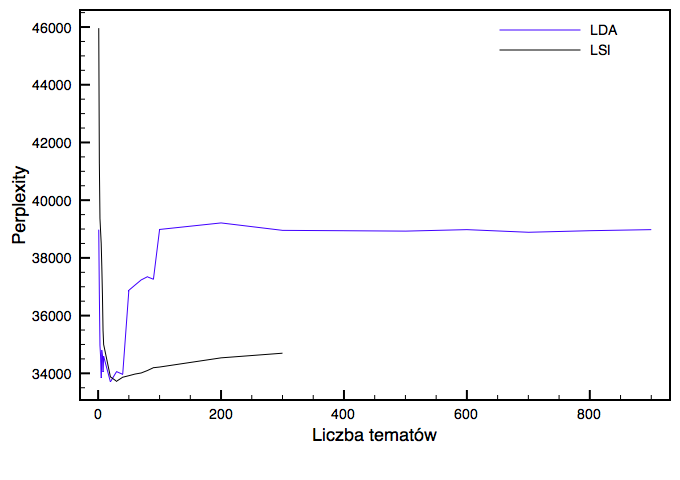
\includegraphics[width=\linewidth]{../doc/gfx/perplexity.png}
\end{frame}

\begin{frame}{Przykładowy problem}
  \pause
  Suma kwadratów ranków skojarzonych dokumentów w zwróconych wynikach z wykorzystaniem CLP
  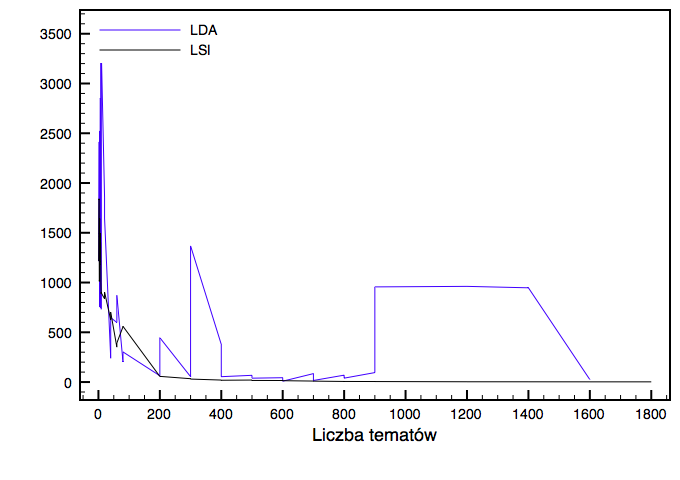
\includegraphics[width=\linewidth]{../doc/gfx/ranks_stemming.png}
\end{frame}

\begin{frame}{Przykładowy problem}
  Suma kwadratów ranków skojarzonych dokumentów w zwróconych wynikach bez wykorzystania CLP
  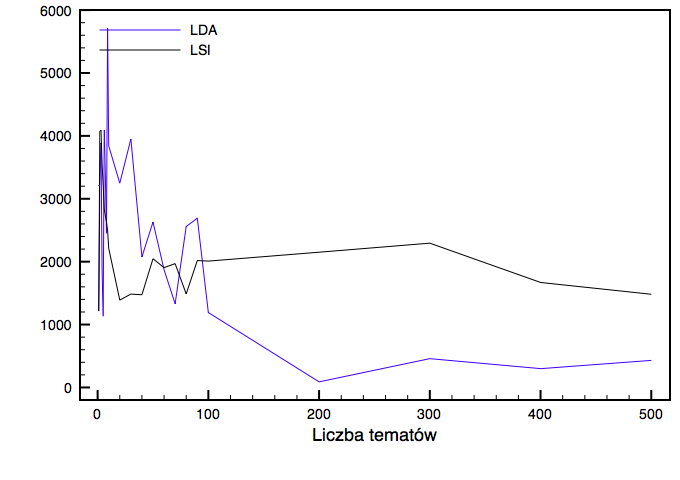
\includegraphics[width=\linewidth]{../doc/gfx/ranks_no_stemming.png}
\end{frame}

\begin{frame}{Wnioski}
  \begin{itemize}
    \pause
    \item LDA spisuje się gorzej niż LSI
    \pause
    \item LDA jest mniej stabilne niż LSI
    \pause
    \item LDA lepiej znosi większy rozmiar słownika
    \pause
    \item LDA lepiej skaluje się z rozmiarami korpusu
  \end{itemize}
\end{frame}
\end{document}
